\documentclass[a4paper, abstracton, DIV=calc, toc=bibliography, toc=listof]{scrreprt}

% silence KOMA warnings about float (for compatibility with listings, algorithm etc.)
\usepackage{scrhack}

% fixes certain things for use with XeTeX
\usepackage{xltxtra}

% language support
\usepackage[ngerman]{babel}

% bibliography
\usepackage[backend=biber, style=alphabetic]{biblatex}
\bibliography{bibliography.bib}

% quotations
\usepackage[strict=true]{csquotes}

% numbers and units
\usepackage{siunitx}

% pseudocode
\usepackage{algpseudocode}
\usepackage{algorithm}

% colors
\usepackage{xcolor}
\colorlet{punct}{red!60!black}
\definecolor{delim}{RGB}{20,105,176}
\colorlet{numb}{magenta!60!black}

% captions and numbering
\usepackage[font=small,labelfont=bf]{caption}
\captionsetup{%
  figurewithin=chapter,
  tablewithin=chapter
}

% listings
\usepackage{listings}
\lstset{
    basicstyle=\ttfamily\scriptsize,
    captionpos=b,
    frame=single,
    aboveskip=1cm
}
\lstdefinelanguage{json}{}
\lstdefinelanguage{pseudo}{}

% line spacing
\usepackage{setspace} 
\setstretch{1.3}

% font stuff
\defaultfontfeatures{Ligatures=TeX}
\setmainfont{Minion Pro}
\setsansfont{Myriad Pro}
\usepackage{dashrule}

% graphics directory
\graphicspath{{assets/}}

% absätze nicht einrücken
\parskip 6pt
\parindent 0pt

% Vermeiden von Schusterjungen und Hurenkindern
\usepackage[all]{nowidow}

% links
\PassOptionsToPackage{hyphens}{url}\usepackage{hyperref}

% good looking tables
\usepackage{booktabs}

%hyphenation rules
\hyphenation{Spread-shirt}

\begin{document}

\pagenumbering{roman}

% title page
\thispagestyle{plain}
\begin{titlepage}
\begin{center}
\includegraphics[width=5cm]{htwk_logo}\\
\vspace{0.3cm}
\normalsize
Fakultät für Informatik, Mathematik und Naturwissenschaften\\
\vspace{2.3cm}
\huge{\textbf{\textsf{Kookkurrenzbasierte Link Discovery am Beispiel von Produkttags}}}\\
\vspace{1cm}
\LARGE{\textsf{Masterarbeit}}\\
\vspace{2.3cm}
\normalsize
Sebastian Marr\\
mail@sebastianmarr.de\\
Leipzig, den 21. November 2013\\
\vspace{2.3cm}
Erstgutachter: Dr. Toralf Kirsten \\
Zweitgutachter: M.Sc. Martin Breest
\end{center}
\end{titlepage}

\begin{abstract}
Durch die Möglichkeit der Benutzerbeteiligung an der Beschreibung, Bewertung und Kategorisierung von Inhalten auf Online-Plattformen werden Begriffswelten aufgebaut, deren Auswertung großes Potenzial für die Verbesserung der Benutzererfahrung bietet. Diese Masterarbeit beschreibt ein Verfahren zum Finden von Zusammenhängen zwischen diesen Begriffen. Grundlage dafür stellen die Daten eines Tagging--Systems und die Ermittlung von Kookkurrenz dar. Die Begriffe und ihre Zusammenhänge werden in eine Graphenrepräsentation transformiert und durch Mining und Integration weiterer Datenquellen angereichert. Zur Priorisierung der Beziehungen für einen Anwendungsfall wird ein Verfahren mittels interaktiver evolutionärer Algorithmen vorstellt und angewendet. Die Ergebnisse der Erzeugung von Beziehungen und der Priorisierung werden präsentiert und schließlich die technische Umsetzung der genannten Verfahren beschrieben.
\end{abstract}
\chapter*{Erklärung}

Hiermit erkläre ich, dass die vorliegende Arbeit von mir selbstständig und nur unter Verwendung der aufgeführten Hilfsmittel erstellt wurde. Alle Stellen, die ich wörtlich oder sinngemäß aus veröffentlichten Schriften entnommen habe, wurden als solche gekennzeichnet. Diese Masterarbeit wurde weder als Ganzes noch in Auszügen für eine andere Prüfung angefertigt.

{
\vspace{32pt}
\noindent
\hdashrule{5cm}{1pt}{1pt 3pt}\\
Sebastian Marr\\
Leipzig, den 21. November 2013
}


\tableofcontents

\cleardoublepage
\pagenumbering{arabic}

\chapter{Einleitung}

Mit der steigenden Menge von nutzergenerierten Inhalten steigt auch die Menge von Metadaten, die mit diesen Inhalten verknüpft sind. Zur späteren Durchsuchbarkeit und Kategorisierung geben viele Online-Plattformen, Marktplätze und Online-Shops ihren Benutzern die Möglichkeit, Inhalte mit Metadaten zu versehen.

Eine oft genutzte Möglichkeit zur Beschreibung von Inhalten sind Tags. Dabei handelt es sich um Wörter oder Wortgruppen, die vom Benutzer frei gewählt werden können, um den Inhalt zu beschreiben. Dabei unterliegt die Eingabe von Tags möglichst wenigen Regeln, um dem Benutzer eine für ihn natürliche Beschreibung des Inhaltes zu ermöglichen. Dabei ist explizit, im Gegensatz zu einer Kategorisierung, die Vergabe von mehreren Tags vorgesehen.

Ein charakteristisches Merkmal von Tags ist dabei, dass sie nur einen bestimmten Aspekt des getaggten Objektes beschreiben. Dabei sind Tags nicht hierarchisch und es werden an keiner Stelle vom Nutzer explizite Zusammenhänge zwischen Tags erstellt. Jedoch liegt die Annahme, dass zwischen Tags Beziehungen herstellbar sind und sich mehrere Tags zu übergeordneten Themen zusammenfassen lassen, nahe. Der Benutzer berücksichtigt diese Beziehungen bei der Eingabe des Tags, formuliert sie jedoch nicht explizit. Die nachträgliche Rekonstruktion der Denkprozesse bei der Eingabe von Tags ist Thema dieser Arbeit.

Dabei ist zu beachten, dass Benutzer bei der Eingabe von Tags unterschiedliche Ziele verfolgen. Idealerweise werden Tags so vergeben, dass sie das getaggte Objekt inhaltlich beschreiben. Jedoch werden vom Benutzer bei der eingabe des Tags weitere Assoziationen hergestellt. Beispielsweise kann der Benutzer mit einem Objekt bestimmte Emotionen oder Wertungen verbinden, die sich in den vergebenen Tags wiederspiegeln.

Auf Marktplätzen, bei denen Verkäufern die Möglichkeit des Taggings ihre Produkte gegeben wird, besteht eine weitere Motivation in der Erhöhung der Auffindbarkeit des Produktes. Dabei kann die inhaltliche Qualität des Tags außer Acht gelassen werden, wenn bei Vergabe einer falschen Beschreibung die Sichtbarkeit des Produktes erhöht wird. Auch der Marktplatzbetreiber selbst kann so vorgehen, um zu versuchen, die Gesamtverkäufe zu steigern.

Die verschiedenen Motivationen der Benutzern von Tags erschwerden die nachträgliche Suche nach Assoziationen. Die vorliegende Masterarbeit beschäftigt sich mit Strategien zur Datenaufbereitung und Nutzung externer und interner Datenquellen und deren Integration mit Tag-Daten. Aus diesen Datenquellen wird eine Datenstruktur mit einem Kookurrenzgraphen als Basis aufgebaut und schließlich werden mit Hilfe von Clustering-Algrithmen daraus Themen extrahiert. Außerdem wird eine Evaluation der Ergebnisse und eine Analyse der verwendeten Methoden durchgeführt.

\section{Motivation und Anwendungen}

Die nachträgliche Herstellung von Assoziationen in vorhandenen Tag-Daten bietet einige Nutzungsmöglichkeiten für den Betreiber der Online-Plattform.

Die Beziehungen zwischen Tags können genutzt werden, um Suchergebnisse zu verbessern. Wenn zu einem Suchbegiff weitere relevante Begriffe bekannt sind, können diese im Suchergebnis mit enthalten sein um somit auch Objekte zu finden, die nicht direkt mit dem Suchbegriff getaggt sind. Außerdem können Suchen vom Benutzer mit Hilfe von verwandten Tags verfeinert werden.

Über die Zusammenfassung von Tags zu Themen lässt sich außerdem die Navigation einer Webseite verbessern. Aus den Themen lassen sich Kategorien oder Hierachien von Kategorien erzeugen, die besser den Denkmustern von Benutzern entsprechen. So sind auch Navigationskonzepte denkbar, die nicht hierarchisch, sondern assoziativ aufgebaut sind. Desweiteren können Tag-Assoziationen für Empfehlungssysteme genutzt werden, die einem Kunden zu einem bestimmten Artikel passende andere Artikel vorschlagen.

Im Bereich des Marketings können Beziehungen zwischen Tags genutzt werden, um für bestimmte externe Suchbegriffe spezielle Seiten zu erstellen (Landing Pages), die Inhalte zu diesem Suchbegriff bereitstellen oder Werbung für diese Suchbegriffe zu schalten. Außerdem können mit Hilfe des Kaufinteresses an bestimmten Themen über die Zeit Trends erkannt werden und mit entsprechenden Marketingmaßnahmen darauf reagiert werden.

All diese Anwendungen führen zu einer besseren Erfahrung für den Benutzer der Plattform. Die Präsentation von Daten kann besser auf die Denkmuster und Erwartungshaltungen des Benutzers angepasst werden. Dies führt in Konsequenz zu einem wirtschaftlichen Vorteil für den Plattformbetreiber.

\section{Kontext}

\section{Aufbau der Arbeit}
\chapter{Problembeschreibung}

Das folgende Kapitel beschäftigt sich mit der Beschreibung der Problemstellung. Dazu wird zuerst das Ziel der Arbeit formuliert. Es folgen grundsätzliche Definitionen und die Beschreibung des zu bearbeitenden Datenbestandes. Abschließend wird die gewählte Lösungsstrategie konzeptionell beschrieben.

\section{Zielstellung}

Das Ziel dieser Arbeit besteht darin, aus vorhandenen Tag-Daten unter Zuhilfenahme von Integration anderer Daten Assoziationen zu extrahieren. Diese Beziehungen sollten im Optimalfall Zusammenhänge widerspiegeln, die zur Verbesserung der Benutzererfahrung beim Suchen nach bestimmten Themen, für Marketingmaßnahmen und generell für ein besseres Verständnis der auf einer Online-Plattform angebotenen Inhalte genutzt werden können.

Nutzbare Beziehungen können vielfältiger Art sein. Denkbar sind beispielsweise

\begin{itemize}
    \item inhaltliche Zusammenhänge, die mittels Clustering-Algorithmen später zu Themengebieten zusammengefasst werden
    \item Worthierarchien, aus denen Kategoriebäume erzeugt werden
    \item Wortformen, die dazu genutzt werden, mehrere Begriffe zusammenzufassen und somit mehr als nur eine wörtliche Suche zu ermöglichen
    \item Verknüpfungen von Wörtern, die über inhaltliche Zusammenhänge hinausgehen, beispielsweise Verbindungen Von Themengebieten mit bestimmten Emotionen, Produkten oder Personen
\end{itemize}

Ausgangsbasis für alle Überlegungen und Berechnungen sind die gesammelten Tag-Daten der Online-Plattform Spreadshirt, deren Struktur und Qualität im nächsten Abschnitt erläutert und diskutiert wird.

\section{Aufbau und Qualität der Daten}

Im folgenden Abschnitt sollen die intern bei Spreadshirt vorhandenen Datenquellen genannt und beschrieben werden. Außerdem wird der Umfang und die Qualität des Datenbestandes diskutiert.

\subsection{Tag-System}
\label{tag-system}

Ein Tag-System besteht im Allgemeinen aus den Mengen \(D\), \(T\) und \(U\). \(D\) bezeichnet die Menge der Dokumente. Ein Dokument \(d\) kann ein beliebiger Datensatz sein, beispielsweise ein Bild, Artikel oder Produkt. Die Menge \(U\) stellt alle Benutzer des Systems dar. Ein Benutzer \(u\) kann neben einem Index weitere Informationen besitzen, die jedoch hier im Kontext des Tag-Systems nicht tiefer gehend behandelt werden. \(T\) ist die Menge der Tags. Ein Tag \(t\) ist eine beliebige Zeichenkette. \(T\) bildet also das \emph{Vokabular} des Tag-Systems.

Die Benutzer können beliebige Dokumente mit beliebigen Tags versehen. Der Vorgang des \emph{Taggens} kann also durch die Relation \(R = D \times U \times T\) beschrieben werden, welche Tupel der Form \((d, u, t)\) enthält.

Der Betreiber der Online-Plattform kann bestimmte Aspekte des Tag-Systems begrenzen. Können alle Benutzer beliebige Tags an beliebigen Dokumente vergeben, spricht man von einer \emph{Folksonomy} \cite{ip2009}.

Im Fall von Spreadshirt ist die Vergabe von Tags auf die Menge der Partner \(P \subseteq U\) begrenzt (siehe auch \ref{spreadshirt}). Die Dokumente, die von den Partnern getaggt werden können, sind auf die Designs und Artikel beschränkt, die der Partner selbst angelegt hat. Eine Beschreibung kann also ausschließlich durch den Autor des Inhaltes erfolgen. Deshalb fehlt im Vergleich zu anderen Tag-Systemen auch die Information, welcher Benutzer den Tag vergeben hat.

Des Weiteren besitzen Tags in der Spreadshirt-Datenbank ein Attribut \emph{Sprache} aus der Menge \(L\). Die Sprache spielt bei der Eingabe und Anzeige der Tags zu Dokumenten eine Rolle. Je nach eingestellter Sprache auf der Webseite erstellt und sieht der Benutzer nur Tags, die mit dieser Sprache markiert sind.

Zum Zeitpunkt der Bearbeitunge dieser Arbeit befanden sich in der Datenbank der europäischen Spreadshirt-Plattform:

\begin{itemize}
    \item \num{2072079} Tags
    \item \num{6433410} Benutzer
    \item \num{26147860} Dokumente (\num{16494430} Artikel und \num{9653430} Designs)
    \item \num{76978414} Taggings
\end{itemize}

In der Menge der Tags befinden sich Tags in \num{15} verschiedenen Sprachen. Es wurden insgesamt \num{71936424} Dokumente mit Tags versehen.

\subsection{Clicktracking}

Spreadshirt betreibt ein Clicktracking-System, welches die Klicks der Benutzer auf Suchergebnisseiten aufzeichnet. Dabei ist unerheblich, ob der Benutzer bei Spreadshirt registriert und angemeldet ist. Dieses System sammelt Daten von beiden Spreadshirt-Plattformen (siehe \ref{platforms}) und erzeugt bei jedem Klick eines Besuchers auf ein Suchergebnis einen Datensatz mit folgenden Attributen:

\begin{itemize}
    \item Suchbegriff
    \item Plattform, \emph{EU} oder \emph{NA}
    \item Zeitstempel des Klicks
    \item ID des geklickten Dokumentes
    \item Position des geklickten Dokumentes auf der Ergebnisseite
    \item Sprache
\end{itemize}

Die Nutzung der Clicktracking-Daten liefert eine andere Sicht auf die Metadaten der Produkte als die Tags. Die Klicks liefern eine Einschätzung des suchenden Benutzers, ob die Metadaten, die für den Suchindex verwendet werden, zum Artikel selbst passen. Die Grundannahme ist hierbei, dass Benutzer nur auf Suchergebnisse klicken, die ihren Erwartungen bezüglich des Suchbegriffes gerecht werden.

Aufgrung der kürzlichen Einführung des Clicktracking-Systems wurde im Kontext dieser Arbeit mit den ersten \num{611836} aufgezeichneten Klicks gearbeitet.

\subsection{Datenqualität}

Die Qualität von Daten wird im Allgemeinen unter mehreren Gesichtspunkten beurteilt \cite{hkp2012}. Dazu gehören unter Anderem \emph{Korrektheit}, \emph{Vollständigkeit}, und \emph{Redundanzfreiheit}. Nachfolgend werden die bei Spreadshirt vorhandenen Daten nach diesen Kriterien betrachtet und die Quellen eventueller Fehler \cite[43 ff]{jo2003} diskutiert.

\paragraph{Korrektheit}

Die Korrektheit der Tag-Daten kann an vielen Punkten angezweifelt werden. Das hervorstechende Problem hierbei ist das Auftreten von Spam. Viele Partner versehen ihre Artikel und Designs mit Tags, die nicht den Inhalt beschreiben. Partner versehen ihre Designs und Artikeln mit falschen Tags, damit diese bei populären Suchbegriffen gefunden werden.

Ein weiterer Defekt ist die Inkorrektheit des Attributes \emph{Sprache} der Tags. Die Sprache wird aus der Domain abgeleitet, die der Benutzer, der den Tag eingegeben hat, besucht hat. Viele Partner geben jedoch ihre Tags in mehreren Sprachen ein, um ihre Inhalte besser auffindbar zu machen. Dies führt in der Konsequenz dazu, dass das Attribut Sprache im großen Teil der Tags als falsch angesehen werden kann.

Die Quelle beider Fehler ist also die bewusste Falscheingabe von Informationen, um einen persönlichen Vorteil zu erlangen.
                                                                                                                                                                                                                                                                                                                                                                                                              
\paragraph{Vollständigkeit}

Wie bereits in \ref{tag-system} beschrieben, fehlen in den Spreadshirt-Daten der Zeitpunkt und der Benutzer eines Taggings. Dies führt in der Konsequenz dazu, dass Spam schwerer erkannt werden kann. Zwar ist bekannt, wann ein Tag das erste Mal verwendet wurde, alle weiteren Verwendungen des Tags werden haben jedoch keinen Zeitstempel. Der Benutzer, der den Tag angelegt und verwendet hat, kann nur daraus abgeleitet werden, wer den getaggten Artikel angelegt hat.

Die Unvollständigkeit der Daten rührt in erster Linie daher, dass zum Zeitpunkt der Implementierung des Tag-Systems noch nicht bedacht wurde, dass die fehlenden Attribute später nützlich sein können.

\paragraph{Redundanzfreiheit}

Bedingt durch die Form der Dateneingabe besteht für das Vokabular des Tag-System ein großes Potential für redundante Daten. Da eingegebene Tags durch einen Separator getrennt eingegeben werden müssen, besteht hier Potential zur Fehleingabe. Wird der falsche Separator verwendet, werden die eigentlich getrennten Tags als eine einzige Entität abgespeichert.

Technisch kann jeder Tag genau ein Mal in der Datenbank vorkommen. Jedoch führen Rechtschreibfehler, unterschiedliche Groß- und Kleinschreibung, verschiedene Arten zusammengesetzte Wörter zu schreiben, Leerräume vor, nach und zwischen Wörtern eines Tags und Tippfehler dazu, dass das gleiche Wort mehrfach in der Datenbank gespeichert wurde.

Außerdem führten in der Vergangenheit Systemfehler und Implementierungsfehler dazu, dass falsche, nicht druckbare Zeichen in den Tags enthalten waren. Nach Beseitigung der Fehler blieben die fehlerhaften Tags bestehen, so dass bei einer erneuten Eingabe des gleichen Wortes ein neuer Tag in der Datenbank angelegt wurde.

\section{Lösungsansatz}
\chapter{Erstellung von Kookkurrenzgraphen}

\section{MapReduce}


\section{Anwendung von MapReduce zur Kookkurrenzberechnung}


Nachdem in diesem Kapitel die theoretischen Grundlagen für die Link Discovery mittels Kookkurrenz beschrieben wurden, beschäftigt sich das folgende Kapitel mit dem technischen System zur Umsetzung des Lösungsansatzes.
\chapter{Systembeschreibung}

Das nachfolgende Kapitel befasst sich mit der Beschreibung der Technologien und Vorgehensweisen, die zur Link Discovery im Rahmen dieser Arbeit angewendet wurden. Dazu zählen im Einzelnen die gewählte Datenbank MongoDB, das Datenmodell des Zielgraphen und das daraus resultierende Vorgehen und die Architektur des Systems zur Link Discovery.

\section{MongoDB}

Zur Umsetzung der Link Discovery wurde das Datenbankmanagementsystem MongoDB \cite{mo2013} gewählt. Bei MongoDB handelt es sich um eine quelloffene dokumentenorientierte Datenbank.

Im Gegensatz zu traditionellen relationalen Datenbanksystemen verzichtet MongoDB dabei auf eine tabellenförmige Struktur der Daten und speichert Datensätze in Form von so genannten \emph{Dokumenten}. Dabei handelt es sich um hierarchische Schlüssel-/Wertpaare, die schemalos in so genannten \emph{Collections} gespeichert werden. Schemalos bedeutet dabei, dass die Dokumente innerhalb einer Collection nicht alle dieselbe Struktur besitzen müssen.

Zur Repräsentation der Dokumente verwendet MongoDB ein Format, dass sich sehr an JSON \cite{json2006} anlehnt. JSON ist ein menschenlesbares Datenaustauschformat, das aus der Objektnotation der Programmiersprache JavaScript abgeleitet wurde. Das Datenformat von MongoDB ist BSON \cite{bson2013}, eine binäre Repräsentation von JSON, die einige zusätzliche Datentypen unterstützt. 

Listing \ref{lst:json} zeigt ein Beispiel für ein Dokument in MongoDB. Das Feld \emph{\_id} ist hierbei ein  Bezeichner vom Typ \emph{ObjectID}. Dieser stellt einen global eindeutigen Bezeichner dar, der benutzt werden kann, um Dokumente zu referenzieren. Innerhalb einer Collection ist \emph{\_id} dabei grundsätzlich eindeutig. Das Feld \emph{address} zeigt, dass Dokumente weitere Dokumente enthalten können. Das Feld \emph{friends} zeigt, dass Werte für Schlüssel auch Arrays von Werten sein können. Diese sind dabei nicht auf primitive Typen wie Zeichenketten oder Zahlen beschränkt, sondern können auch weitere Dokumente sein.

\begin{lstlisting}[language=json, label={lst:json}, caption={Ein Beispiel für ein Dokument in MongoDB}]
{
    "_id" : ObjectId("51efc20147cae77dfc02e0ac"),
    "name" : "Bob",
    "age": 25,
    "address": {
        "city": "Leipzig",
        "street": "Karl-Liebknecht-Str. 132"
        "zip": "04277"
    },
    "friends" : [
        "alice",
        "fred",
        "jason"
    ]
}
\end{lstlisting}

MongoDB unterstützt Anfragen über ein Binärprotokoll, welches über so genannte \emph{Treiber} in vielen Programmiersprachen abstrahiert zur Verfügung steht. Dabei sind vielfältige Lese- und Schreiboperationen möglich, die komplexe Abfragen und Operationen auf den gespeicherten Daten zulassen. Außerdem bietet MongoDB eine Implementierung des MapReduce-Programmiermodells (siehe \ref{mapreduce}) sowie die Möglichkeit, Indizes auf allen Hierarchieebenen der Dokumente zu nutzen. Für interaktive Operationen steht die \emph{Mongo Shell} zur Verfügung, welche Abfragen mittels der Programmiersprache JavaScript erlaubt und somit einen Treiber für diese Sprache darstellt.

Aufgrund der genannten Eigenschaften stellt MongoDB einen exzellenten Ausgangspunkt für die Link Discovery im Rahmen dieser Arbeit dar. Durch die vorhandene Schemaflexibilität können die Daten in der gerade benötigten Form gespeichert und abgefragt werden. Durch die Unterstützung von MapReduce mit mehreren Rechnern lassen sich Berechnungen wie die der Kookkurenz (siehe \ref{mapreduce_cooccurence}) parallelisieren und somit beschleunigen.

Aus diesen Gründen stellt MongoDB das zentrale technische Element für die Link Discovery im Rahmen dieser Arbeit dar. Sobald die Daten aus den externen und internen Quellen in MongoDB importiert wurden, können die folgenden Schritte direkt mit Datenbankabfragen realisiert werden.

\section{Datenmodell}

Nach der Auswahl eines geeigneten Datenbanksystems sollte das Datenmodell des Ergebnisses genauer spezifiziert werden. Ist dieses vor der Link Discovery klar, können die einzelnen benötigten Schritte zur Erreichung des Zieles einfacher definiert werden.

Generell handelt es sich bei dem gewünschten Ergebnis um einen gerichteten Multigraph. Dieser repräsentiert Objekte, oder auch \emph{Knoten}, zwischen denen paarweise Verbindungen, die \emph{Kanten} bestehen. Die Besonderheit eines Multigraphen ist dabei, dass zwischen zwei Knoten auch mehrere Kanten existieren dürfen \cite{rd2012}. Dies ist dem gewählten Lösungsansatz geschuldet, da zwischen Wörtern und Wortgruppen verschiedenartige Beziehungen existieren können.

Somit müssen für das Datenmodell die beiden Entitäten \emph{Knoten} und \emph{Kante} modelliert werden.

\subsection{Knoten}

Die Knoten repräsentierendie Wörter und Wortgruppen zwischen denen durch Link Discovery Verbindungen hergestellt werden sollen. Sie enthalten als benötigte Attribute eine Zeichenkette und ein Attribut Sprache. Die Kombination dieser beiden Attribute ist innerhalb der Knotenmenge eindeutig. Außerdem erhält jeder Knoten zur einfacheren Referenzierung einen eindeutigen Bezeichner.

Neben diesen immer vorhandenen Attributen kann ein Knoten beliebig viele weitere Eigenschaften besitzen. Diese Eigenschaften dienen dazu, den Begriffen, die die Knoten existieren, für spätere Verwendungen zusätzlichen Kontext zu geben. Im Wesentlichen definieren sich diese zusätzlichen Eigenschaften aus den Datenquellen, die zum Zweck der Link Discovery in den Graph integriert werden.

Zur besseren Kapselung und Übersicht sollten die zusätzlichen Eigenschaften in weitere Entitäten gekapselt werden. Die Struktur dieser zusätzlichen Typen kann dann zum Zeitpunkt der Integration der jeweiligen Datenquelle definiert werden.

Das resultierende Knotenmodell ist in Abbildung \ref{fig:node_erd} dargestellt.

\begin{figure}
\label{fig:node_erd}
\begin{center}
    \includegraphics[width=0.6\textwidth]{node_erd}
\end{center}
\caption{Knotenmodell als Entity-Relationship-Diagramm}
\end{figure}

\subsection{Kanten}



\subsection{Technische Umsetzung}

\begin{figure}
\label{fig:graph_model}
\begin{center}
    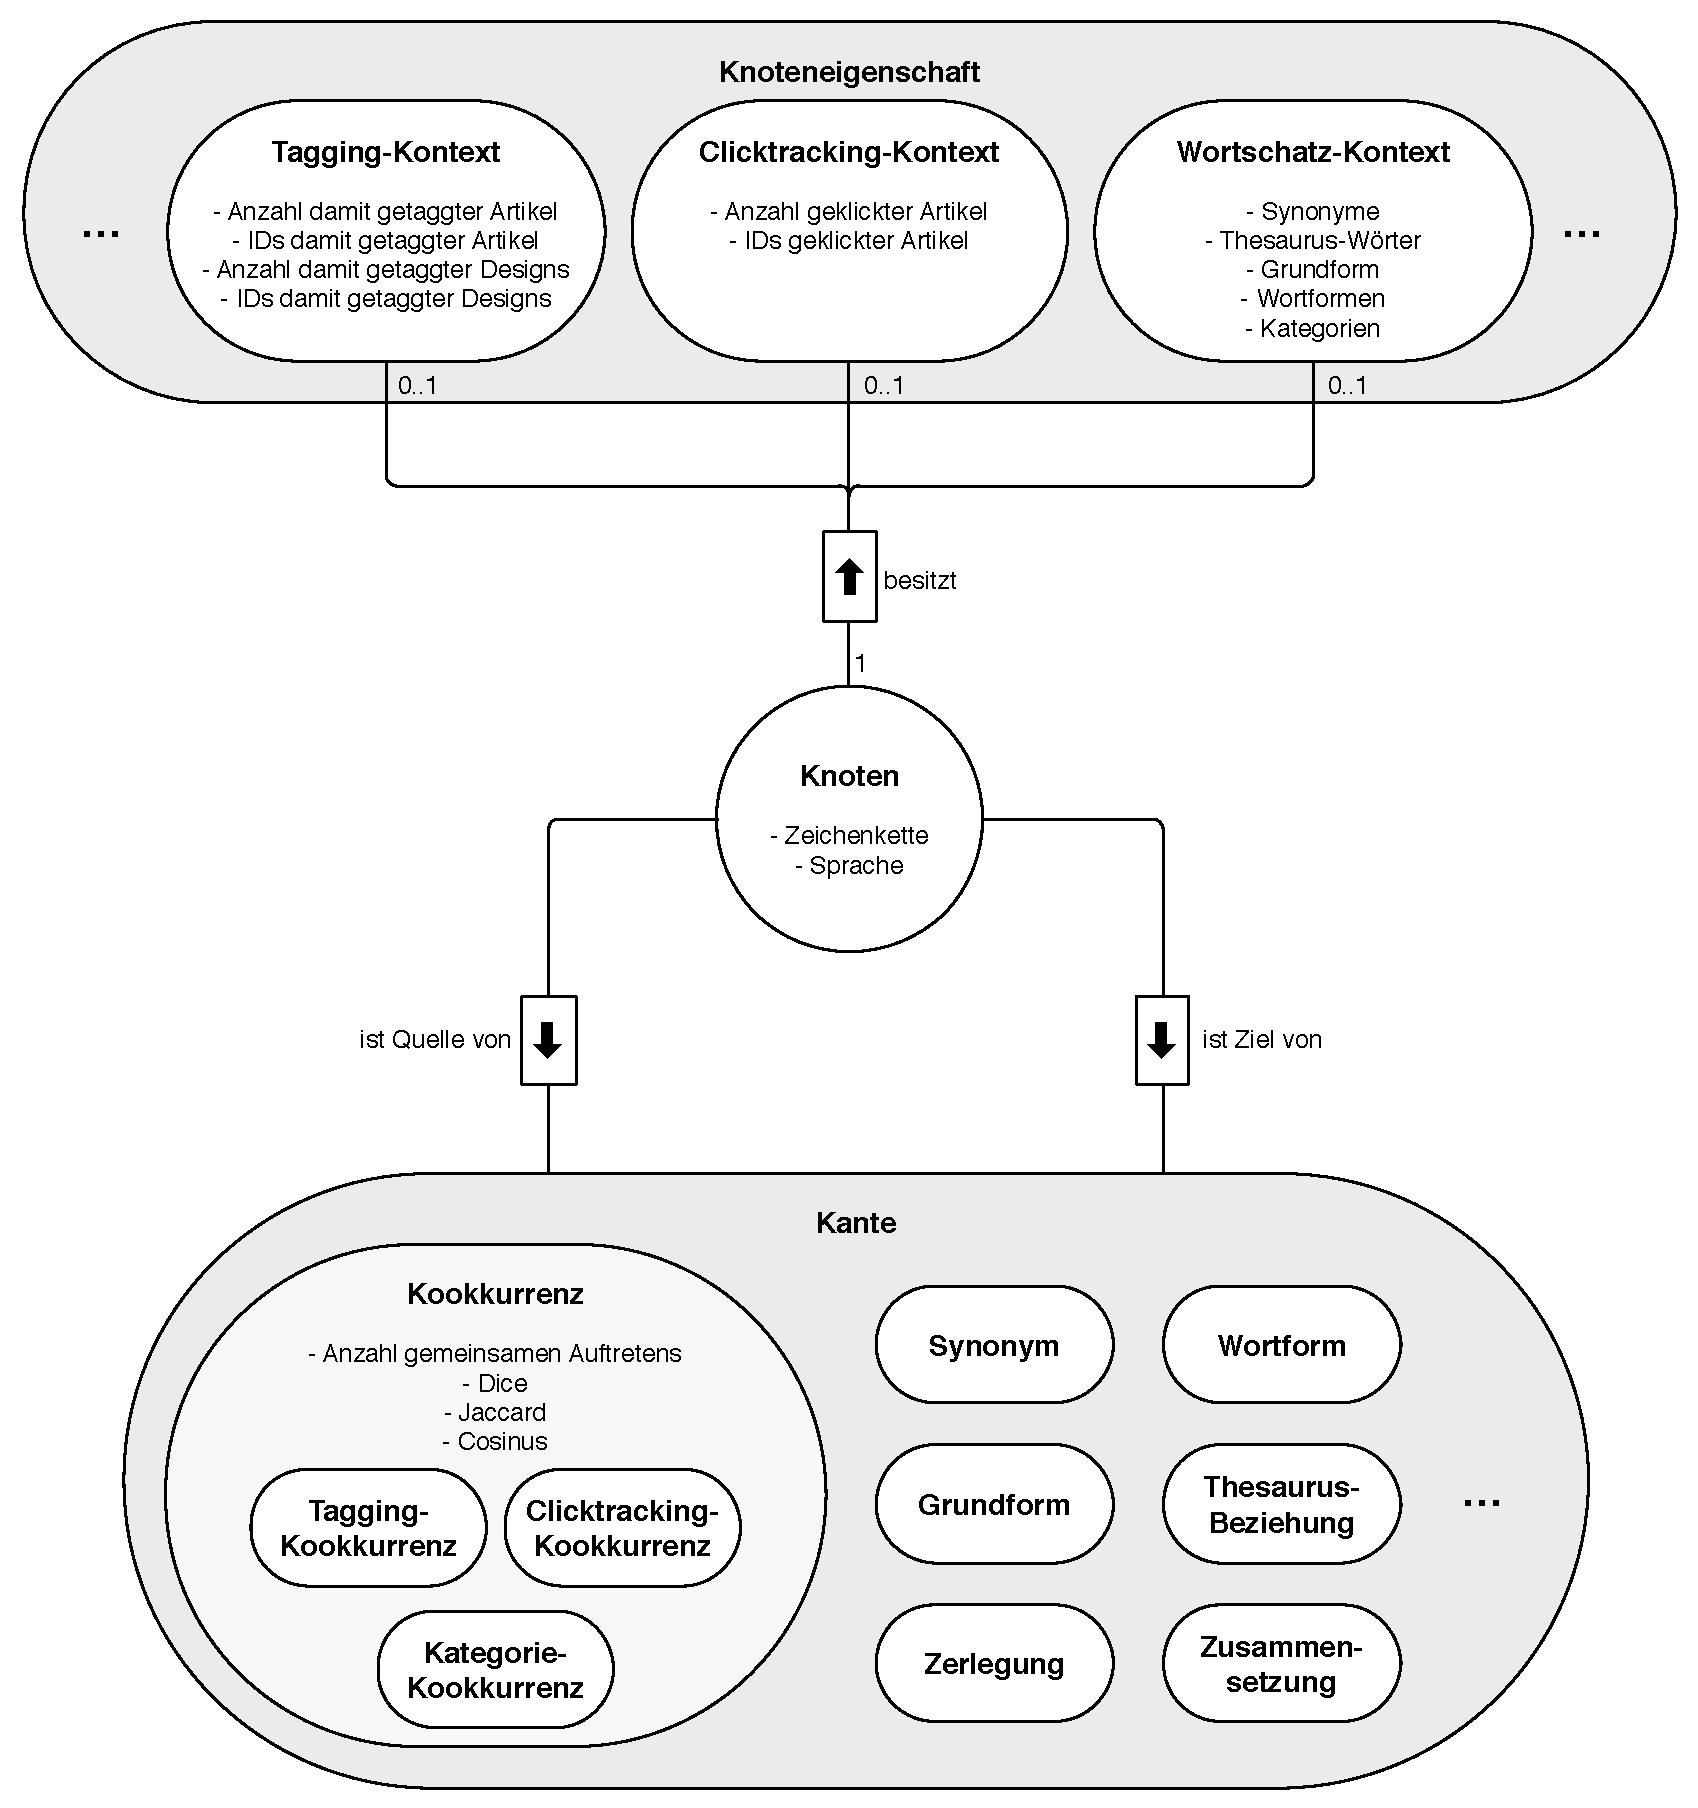
\includegraphics[width=1\textwidth]{graph_model}
\end{center}
\caption{Datenmodell des Graphen als Entity-Relationship-Diagramm}
\end{figure}

\section{Systemarchitektur}

\begin{figure}
\label{fig:architecture}
\begin{center}
    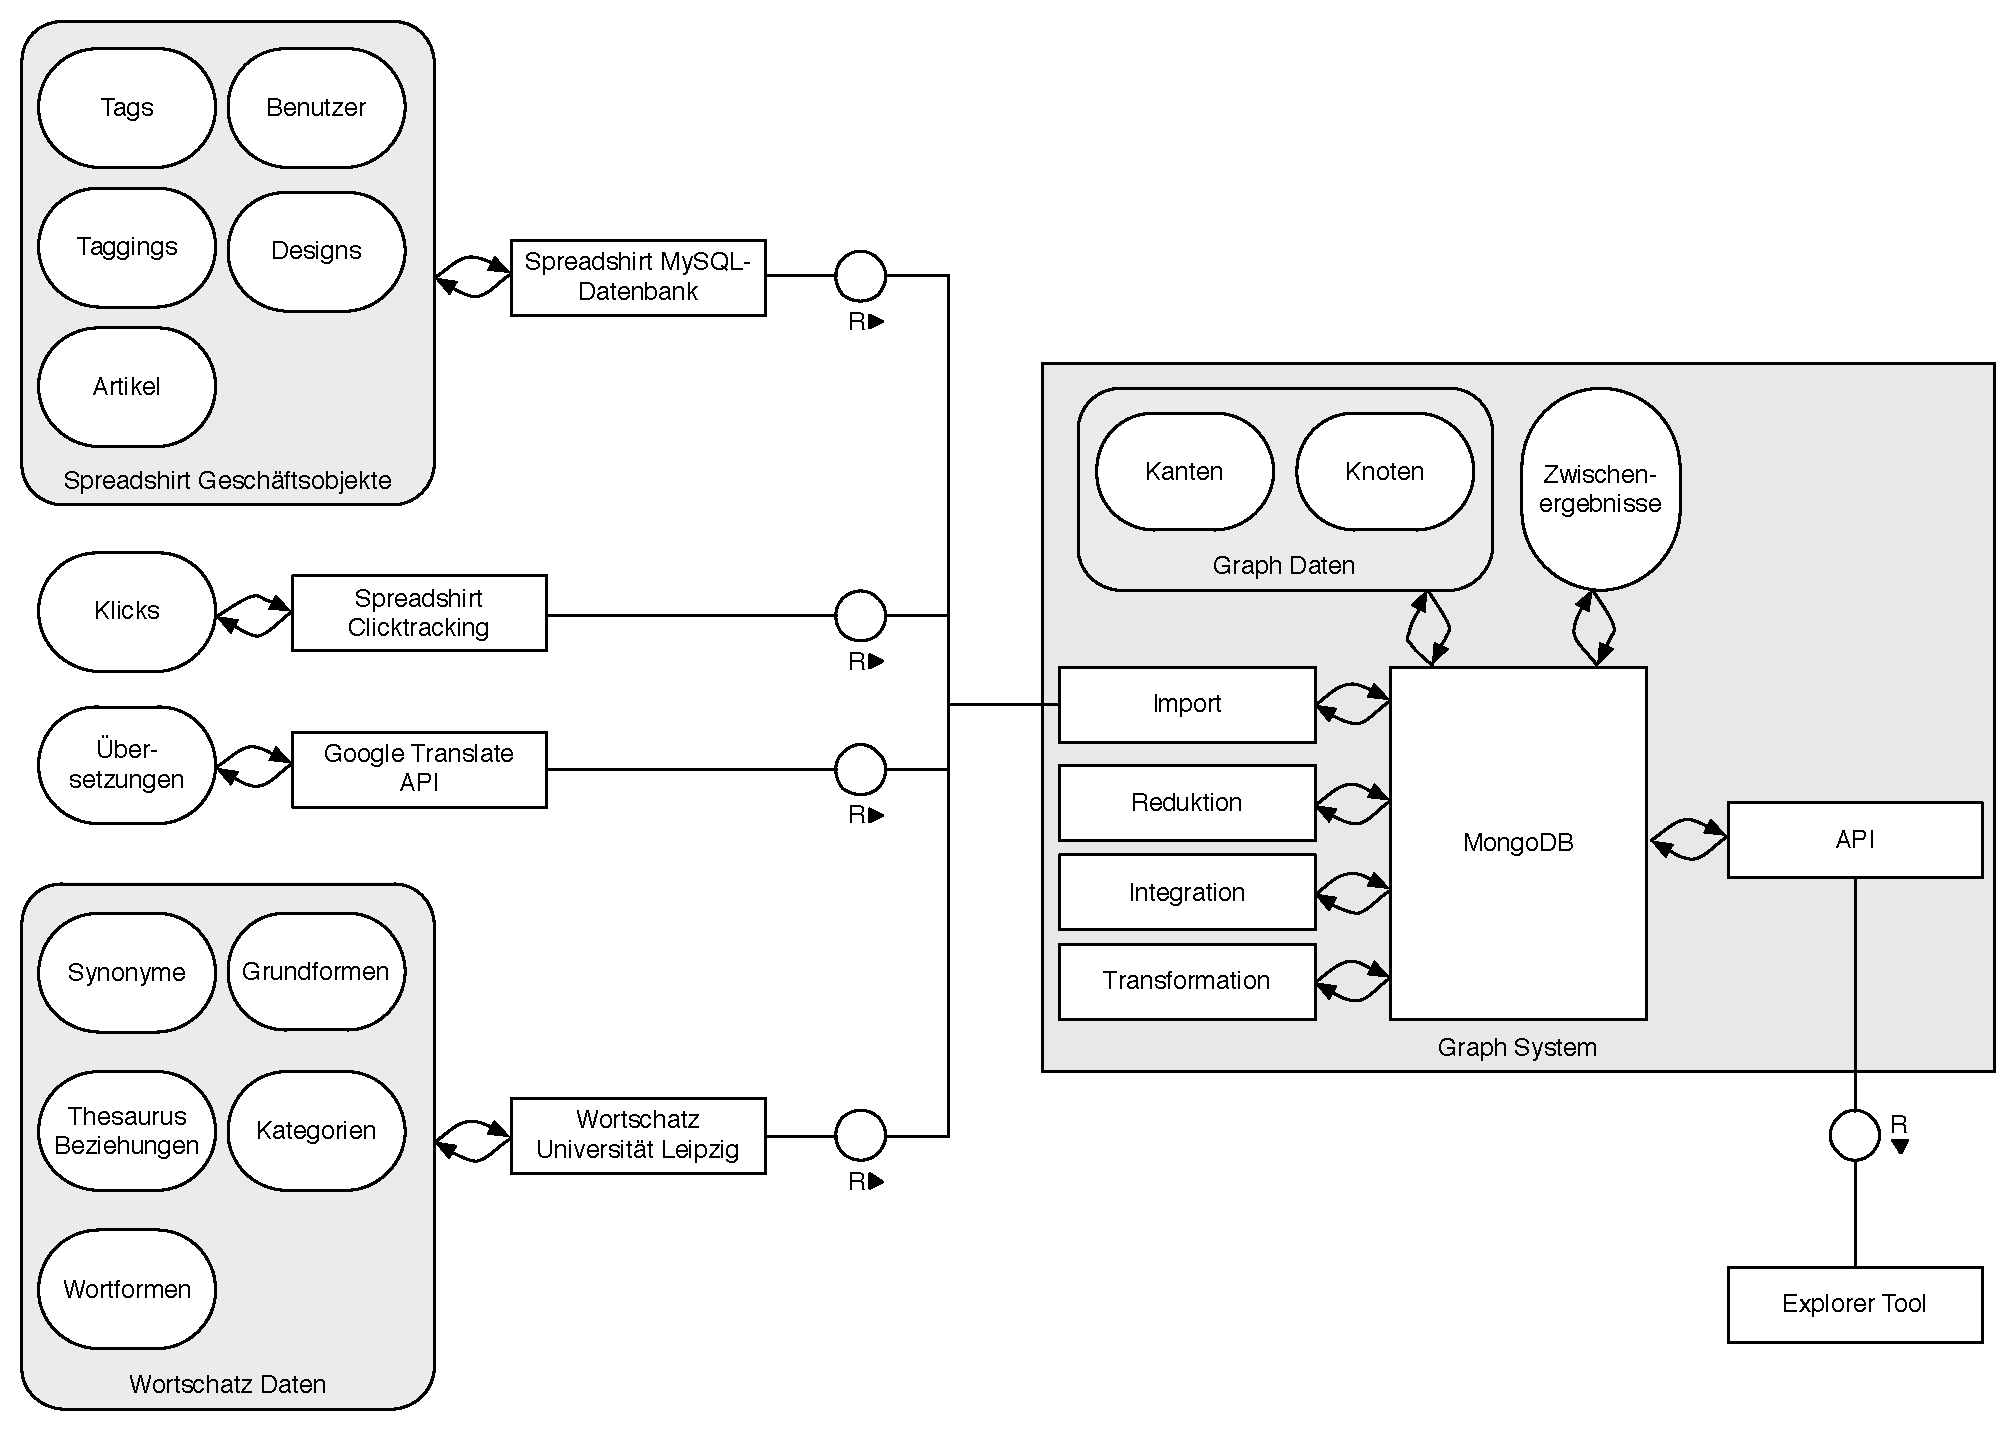
\includegraphics[width=1\textwidth]{architecture}
\end{center}
\caption{Systemarchitektur}
\end{figure}

\chapter{Link Discovery}

Das folgende Kapitel beschäftigt sich mit den im Rahmen dieser Arbeit unternommenen Schritten zur Link Discovery, also dem Finden von Beziehungen zwischen Wörtern und Wortgruppen. Dazu zählen die Generierung eines Ausgangsgraphen aus Tag-Daten sowie dessen Anreicherung durch die Integration weiterer interner und externer Datenquellen.

\section{Tags}

Den Ausgangspunkt für den in \ref{solution} beschriebenen Lösungsansatz stellen die Daten des Tag-Systems dar. Diese werden in \ref{tag-system} ausführlich beschrieben. Aus diesen Daten wird im ersten Schritt der Graph erstellt, in diesen in allen weiteren Schritten weitere Daten integriert werden. Die in diesem Graph enthaltenen Knoten stellen also die Kriterien für die Abfrage der weiteren Datenquellen dar.

Um den Ausgangsgraphen zu berechnen, sind die Schritte des Imports, der Bereinigung, der Reduktion, der Transformation und der Integration notwendig \cite{hkp2012}, welche im folgenden genauer beschrieben werden.

\subsection{Import}

Die Daten liegen im Quellsystem in relationaler Form vor. Somit existieren Tabellen für die Tags, Dokumente und Verknüpfungen zwischen ebenjenen. Da der Inhalt der Dokumente nicht relevant für die Link Discovery mittels Kookkurenz sind, genügt es, die Tabellen der Tags und Verknüpfungen zu importieren.

Die Tags liegen in der Form \((i, s, l)\) vor, wobei \(i\) den eindeutigen Bezeichner des Tags, \(s\) die Zeichenkette und \(l\) die Sprache des Tags repräsentieren.

Die Verknüpfungen sind durch Tupel der Form \((i, t, d_t, d_i)\) repräsentiert, wobei \(i\) der eindeutige Bezeichner der Verknüpfung selbst ist. \(t\) ist der Bezeichner des Tags, \(d_t\) der Typ des Dokuments und \(d_i\) der Bezeichner des Dokumentes. \(d_t\) und \(d_i\) bilden also den zusammengesetzten Schlüssel des getaggten Dokumentes. 
 
\begin{figure}
\centering
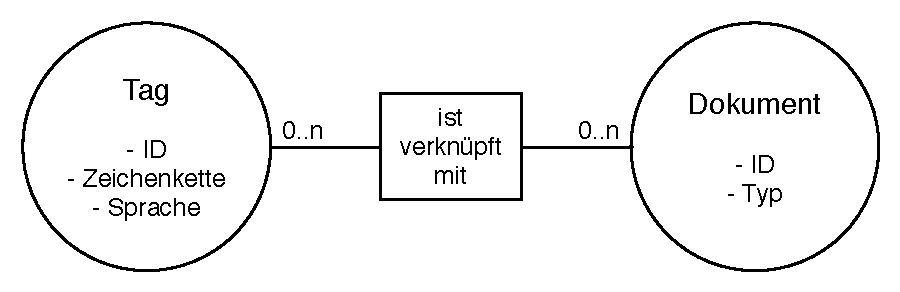
\includegraphics[width=0.6\textwidth]{tag_source_erd}
\caption{Tag-Quelldaten als Entity-Relationship Diagramm}
\label{fig:tag_source_erd}
\end{figure}

Die importierten Quelldaten sind in Abbildung \ref{fig:tag_source_erd} als Entity - Relationship Diagramm abgebildet. Nach dem Import stehen \num{2072079} Tags und \num{71938905} Verknüpfungen zur Verfügung.

\subsection{Bereinigung}

An den Tag-Daten liegen die in \ref{quality} genannten Defekte in Hinblick auf die Datenqualität vor. Diese sollten in einem Bereinigungsschritt reduziert werden. Hierbei liegt das Hauptaugenmerk auf der Erkennung von Duplikaten und später nicht verwertbaren Zeichenketten. Alle durchgeführten Maßnahmen zur Bereinigung beziehen sich hierbei auf die Eigenschaft \(s\) des Tags, also der Zeichenkette selbst.

In den unbereinigten importierten Daten existieren keine Duplikate in der Art, dass eine Paarung aus Zeichenkette und Sprache immer nur genau einmal in den Daten vorhanden ist. Jedoch enthalten viele der Tags nicht weiter verwertbare Zeichen wie nicht druckbare ASCII Zeichen, Anführungszeichen, Satzzeichen, Sonderzeichen sowie überflüssige Leerzeichen am Anfang und Ende der Zeichenkette. Außerdem existiert in den importierten Daten eine Unterscheidung zwischen Groß- und Kleinschreibung. Diese Unterscheidung bringt im Kontext der Link Discovery keine Vorteile und kann somit entfernt werden.

\begin{table}
\centering
\begin{tabular}{|l|l|}
    \hline
    Rohdaten & Bereinigte Daten \\
    \hline
    \textbackslash u0003\textbackslash r\textbackslash nregenbogen & regenbogen \\
    RegenBogen & regenbogen \\
    "Regenbogen" & regenbogen \\
    regenbogen +einhorn & regenbogen einhorn\\
    \hspace{10 mm} regenbogen & regenbogen \\
    regenbogen & regenbogen \\
    \hline
\end{tabular}
\caption{Beispiele für die Tag-Bereinigung}
\label{tab:tag_cleaning}
\end{table}

Somit besteht der Bereinigungsschritt darin, nicht verwertbare Zeichen zu entfernen und alle Großbuchstaben in Kleinbuchstaben umzuwandeln. Dadurch entstehen Duplikate, welche im darauf folgenden Reduktionsschritt entfernt werden können. In Tabelle \ref{tab:tag_cleaning} sind einige Beispiele für die Bereinigungen aufgeführt. Dabei ist gut zu erkennen, dass durch die Bereinigungen Duplikate erzeugt werden.

\subsection{Reduktion}

Der Reduktionsschritt dient zur Einschränkung der Gesamtdaten auf eine nützliche oder handhabbare Menge. Außerdem kann durch Reduktion auch die Datenqualität verbessert werden.

Im Fall der Tag-Daten liegt das Hauptaugenmerk im Reduktionsschritt auf der Entfernung von Duplikaten, die bei der Bereinigung entstanden sind. Dabei muss gleichzeitig sicher gestellt werden, dass keine Informationen über die Verwendung der Tags verloren gehen. Somit besteht die Duplikatentfernung der Tags im Zusammenführen von Datensätzen mit gleichen Zeichenketten und Sprachen. Dabei werden auch die Verwendungen der Tags zusammengeführt.

Werden die Verknüpfungen zweier Tags mit Dokumenten zusammengeführt, können auch dabei wieder Duplikate entstehen. Diese müssen in diesem Fall entfernt werden, da ein Tag nicht mehrmals mit einem Dokument verknüpft werden kann. Das Zusammenfühen von Tags ist exemplarisch in Abbildung \ref{fig:tag_reduction} dargestellt.

\begin{figure}
\centering
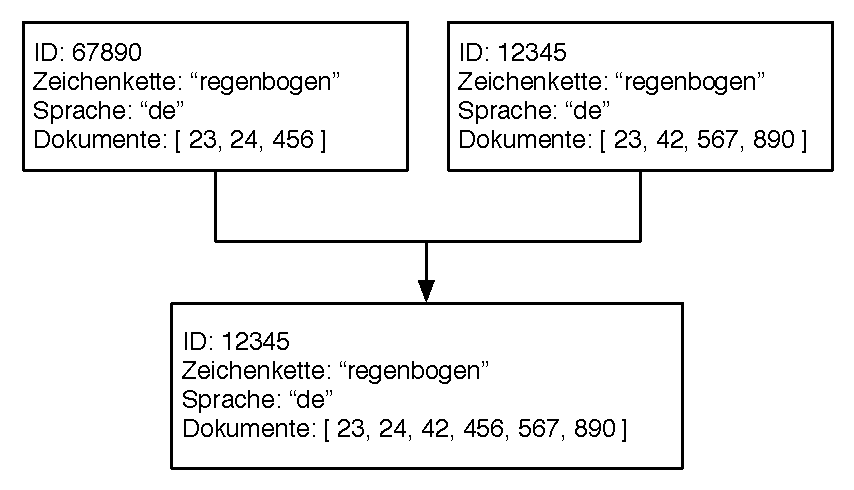
\includegraphics[width=0.7\textwidth]{tag_reduction}
\caption{Beispiel für das Zusammenführen der bereinigten Tags}
\label{fig:tag_reduction}
\end{figure}

Eine weitere im Rahmen dieser Arbeit unternommene Maßnahme zur Datenreduktion bestand darin, sich auf die Menge der Tags zu beschränken, deren Attribut \(l\) den Wert \emph{de} besitzt. Praktisch handelt es sich dabei um alle Tags, die als deutsch gekennzeichnet in der Datenbank gespeichert sind. Diese Einschränkung wurde vorgenommen, um die zu verarbeitende Datenmenge überschaubar zu halten.

Ein letzter Reduktionsschritt besteht in der Entfernung der Tags, deren Zeichenketten eine Länge von \num{1} besitzen, da in der deutschen Sprache keine einbuchstabigen Wörter existieren.

Nach der beschriebenen Reduktion befinden sich noch \num{314351} Tags und \num{23255714} Verknüpfungen in der Datenbank. Dies entspricht einer Reduktion von ca. \num{68} Prozent gegenüber der importierten Menge von Objekten.

\subsection{Transformation}

Der Transformationsschritt beschreibt die Überführung der Daten in die Form, die für das Ergebnis benötigt wird. Im Falle der Tag-Daten bedeutet dies eine Umformung in die Form des Kokkurrenzgraphen, also die Erzeugung von Knoten- und Kantenobjekten. Die Umsetzung dieser Transformation mittels des Programmiermodells MapReduce wurde in \ref{mapreduce_cooccurence} genauer beschrieben.

Um die vorhandenen Informationen später einfach nutzbar zu machen, erscheint es sinnvoll, die Knoten mit allen verfügbaren Daten anzureichern. Dazu gehören bei den Tags die Sprache und Zeichenkette, sowie Informationen darüber an welche Dokumente der Tag verwendet wurde. Diese Informationen lassen sich in einer dokumentenbasierten Datenbank leicht abbilden.

Je Tag wird ein Datenbankdokument erzeugt, dass den Knoten repräsentiert. Dieses besitzt als Attribute zum einen die Zeichenkette und die Sprache des Tags, aus dem es erzeugt wurde. Zum anderen wird ein Unterdokument hinzugefügt, welches weitere Eigenschaften des Ausgangstags beschreibt. Die umfasst die Anzahl der Verwendungen und die eindeutigen Bezeichner der Dokumente, die mit dem Tag getaggt wurden. Außerdem kann im Transformationsschritt für jeden Knoten ein global eindeutiger Bezeichner erzeugt werden, um das spätere Referenzieren der Knoten einfacher zu machen. Zeichenkette und Sprache des Knotens stellen einen zusammengesetzten Schlüssel dar und sind in der Knotenmenge eindeutig. Der Aufbau der Knoten ist schemahaft in Abbildung \ref{fig:tag_transform_node} dargestellt. Listing \ref{lst:tag_transform_node} zeigt ein Beispiel für ein in der Datenbank abgelegtes Knotendokument.

\begin{figure}
\begin{center}
    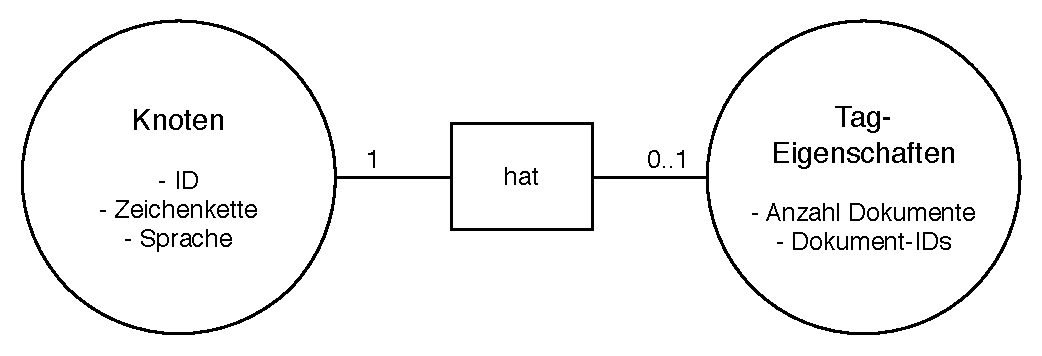
\includegraphics[width=0.7\textwidth]{tag_transform_node}
\end{center}
\caption{Aufbau der aus den Tag-Daten erzeugten Knoten}
\label{fig:tag_transform_node}
\end{figure}

\begin{lstlisting}[language=json, label={lst:tag_transform_node}, caption={Tag-Knoten als JSON-Dokument}]
{
    "_id" : ObjectId("51efc20147cae77dfc02e0ac"),
    "language" : "de",
    "string" : "mama",
    "tagProperties" : {
        "occurenceCount" : 3,
        "articleCount" : 2,
        "designCount" : 1,
        "articleIDs" : [
            24231101,
            24231105
        ],
        "designIDs" : [
            15514592
        ]
    }
}
\end{lstlisting}

Die Erzeugung der Kanten erfolgt dann wie in Abschnitt \ref{mapreduce_cooccurence} beschrieben. Dabei werden für jedes gemeinsame Auftreten von zwei Tags zwei Datenbankdokumente erzeugt. Dieses beschreiben gerichtete Kanten zwischen den Tags, die ein gemeinsames Auftreten der Tags repräsentieren. Neben Quell- und Zielknoten enthält eine Kante den Kantentyp sowie weitere Informationen über die Art der Verbindung. Im Fall von Kookkurenzkanten ist dies zum einen die absolute Anzahl gemeinsamer Vorkommen der Tags, zum anderen die in \ref{measures} beschriebenen Kookkurenzmaße. Der Kantentyp ist aus der Berechnung folgend der Typ der Tag-Kookkurenz. Der Aufbau der erzeugten Kanten ist in Abbildung \ref{fig:tag_transform_edge} dargestellt. Ein Beispiel JSON-Dokument für eine Kante ist in Listing \ref{lst:tag_transform_edge} zu sehen.

\begin{figure}
\centering
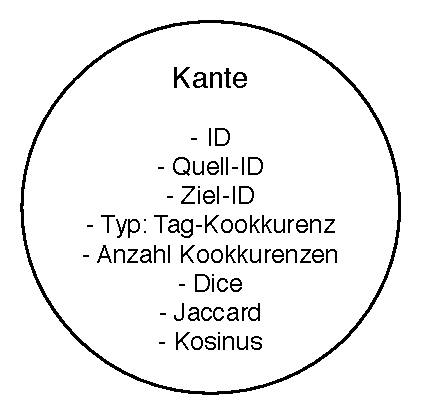
\includegraphics[width=0.3\textwidth]{tag_transform_edge}
\caption{Aufbau der aus den Tag-Daten erzeugten Kanten}
\label{fig:tag_transform_edge}
\end{figure}

\begin{lstlisting}[language=json, label={lst:tag_transform_edge}, caption={Tag-Kante als JSON-Dokument}]
{
    "_id" : ObjectId("51efd6f61177ff360605bd99"),
    "source" : ObjectId("51efc1af47cae77dfc00c3f8"),
    "target" : ObjectId("51efc1e047cae77dfc02087c"),
    "type" : "tag-co-occurence",
    "occurences" : 1,
    "dice" : 0.0001317089232795522,
    "jaccard" : 0.00006585879873551106,
    "cosine" : 0.008115343414514944
}
\end{lstlisting}

\subsection{Integration}

Da der aus den Tag-Daten generierte Kookkurenzgraph die Ausgangsbasis für alle weiteren Operationen darstellt, muss im Sinne der Integration nichts getan werden. Die transformierten Daten müssen lediglich in die Zieldatenbank kopiert werden.

Durch die Schritte, die zur Link Discovery aus den Tag-Daten verwendet wurden, wurden insgesamt \num{314351} Knoten und \num{21834868} Kanten erzeugt, welche nun durch weitere Schritte angereichert werden sollen.

\section{Clicktracking}

Wie in \ref{problem:clicktracking} bereits einführend beschrieben, betreibt Spreadshirt ein Clicktracking-System, welches die Klicks der Benutzer auf Suchergebnisseiten aufzeichnet. Die von diesem System erzeugten Daten können für die Link Discovery von großer Bedeutung sein, da sie eine andere Perspektive auf die Begriffe im Graphen liefern. Die Tags liefern die Sicht der Partner, also der Personen, die Inhalte hochladen und verkaufen möchten. Die Klicks beschreiben die Sicht der Käufer, also der Personen, die nach Inhalten suchen. Durch die Auswertung der Clicktracking-Daten ergibt sich also die Möglichkeit, eine Form der Validierung der durch Partner vergebenen Metadaten zu erhalten. Die Annahme hierbei ist, dass Käufer nur auf Suchergebnisse klicken, die eine inhaltliche Relevanz zum eingegebenen Suchbegriff besitzen.

Wie bereits für die Tag-Daten, werden im Folgenden auch für das Clicktracking die Schritte Import, Bereinigung, Reduktion, Transformation und Integration näher erläutert. Der Ansatz zur Erzeugung der Verbindungen ist ebenfalls kookkurenzbasiert.

\subsection{Import}
\label{click_import}

Das Clicktracking-System erzeugt Dateien im JSON-Format, die zu jedem Klick auf einer Ergebnisseite die wesentlichen Informationen enthalten. Dabei ist pro Klick ein JSON-Dokument in der Datei abgespeichert. Ein Beispiel für ein solches Dokument ist in Listing \ref{lst:click_raw} dargestellt.

\begin{lstlisting}[language=json, label={lst:click_raw}, caption={Clicktracking - Rohdokument als JSON}]
{
    "date": "01.07.2013 00:09:31_633",
    "path": "/track/eu/205909/1E3B6E3E-B454-4496-C51A14A8FA25/2.10.4/list",
    "params": {
        "locale": "[de_DE]",
        "search-query": "[biene]",
        "cl": "[a18869874, p25446183, i49]"
    }
}
\end{lstlisting}

Ein Clicktracking-Dokument enthält dabei die Attribute \emph{Datum}, \emph{Pfad}, \emph{Gebietsschema}, \emph{Suchbegriff} und die Daten des eigentlichen Klicks, also den geklickten \emph{Artikel}, das geklickte \emph{Produkt} und den \emph{Index}, also die Position des geklickten Inhaltes auf der Suchergebnisseite. Die Unterscheidung zwischen Produkt und Artikel ist dabei im Domänenmodell von Spreadshirt begründet und für die Link Discovery nicht von Interesse. Es genügt, den geklickten Artikel im Weiteren näher zu betrachten.

Auffällig ist, dass die Möglichkeiten des JSON-Formates bei der Speicherung der Klickdaten nicht vollständig ausgenutzt wurden. So sind die Werte, die das geklickte Dokument beschreiben, als Zeichenkette abgelegt und zusätzlich die eindeutigen Bezeichner mit einem Buchstaben versehen, der ihren Typ angibt. Des weiteren enthalten  das Gebietsschema und der Suchbegriff zusätzliche eckige Klammern. Diese Defekte sollten im Bereinigungsschritt beseitigt werden, um ein nutzbareres Datenformat zu erhalten.

Da das Clicktracking-System zum Zeitpunkt des Imports erst 3 Monate Daten aufzeichnete, standen \num{2249942} solcher Klickdokumente zur Verfügung.

\subsection{Bereinigung}

Im Bereinigungsschritt müssen zunächst die genannten Defekte der Klickdaten beseitigt werden. Dazu gehört die Entfernung der eckigen Klammern in Suchbegriff und Gebietsschema und die Extraktion des eindeutigen Bezeichners des geklickten Artikels. Aus dem Gebietsschame ist nur die Sprache von Interesse. Außerdem wurden für den Suchbegriff die gleichen Bereinigungsoperationen wie für die Tag-Daten vorgenommen, also die Entfernung von überflüssigen Leerzeiche, Groß-/Kleinschreibung, nicht druckbarer Sonderzeichen und Satzzeichen.

Im Bereinigunsschritt werden so auch einfacher verarbeitbare Dokumente erzeugt, da die Möglichkeiten des JSON-Formates besser ausgenutzt werden. Listing \ref{lst:tag_cleanup} zeigt das Ergebnis der Bereinigung des in \ref{click_import} gezeigten Beispieldokumentes.

\begin{lstlisting}[language=json, label={lst:tag_cleanup}, caption={Bereinigtes Clicktracking-Dokument}]
{
    "_id": ObjectId("51e7b1e0417498f9c6868939"),
    "query" : "biene",
    "date" : "2013-07-01T00:09:31.633Z",
    "articleId" : 18869874,
    "index" : 57,
    "language" : "de"
}
\end{lstlisting}

\subsection{Reduktion}

Die Reduktion der Clicktracking-Daten besteht zum einen aus einer Duplikatentfernung, zum anderen aus der Einschränkung der Sprache.

Im Sinne der Kookkurenz ist es nicht von Bedeutung, wenn Paare aus Suchbegriffen und geklickten Artikeln mehrfach auftauchen, da hierfür nur das gemeinsame Auftreten unterschiedlicher Suchbegriffe betrachtet wird. Somit besteht die Duplikatentfernung lediglich darin, aus mehrfach vorkommenden Artikel-/Klickpaaren genau eines auszuwählen.

Außerdem erfolgte, wie schon bei den Tag-Daten, eine Einschränkung auf Klicks, die als \emph{deutsch} gekennzeichnet sind.

Nach dem Reduktionsschritt verblieben zur Transformation noch \num{411341} Klicks.

\subsection{Transformation}

Im Transformationsschritt wird für die Clicktracking-Daten ein Kookkurrenzgraph berechnet. Die Kookkurrenz bestimmt sich hierbei daraus, welche Suchbegriffe zum Klick auf einen Artikel geführt haben. Wird ein Artikel zu mehreren Suchbegriffen geklickt, liegt die Vermutung nah, dass zwischen den Suchbegriffen ein irgendwie gearteter Zusammenhang besteht.

Ziel der Transformation ist somit die Erzeugung von Knoten und Kanten. Die Knoten besitzen dabei zusätzliche Eigenschaften, die die Eigenschaften des durch den Knoten repräsentierten Begriffes im Kontext des Clicktrackings widerspiegeln. Konkret sind dies die Artikel, die zu dem Begriff als Suchbegriff geklickt wurden. Listing \ref{lst:click_node} zeigt beispielhaft ein erzeugtes Knotendokument.

\begin{lstlisting}[language=json, label={lst:click_node}, caption={Knotendokument mit Clicktracking-Eigenschaften}]
{
    "_id": ObjectId("51e7f1e04146498f9c6868945"),
    "string": "biene",
    "language": "de",
    "clickProperties": [
        { "articleId": 4512 },
        { "articleId": 4794 },
        ...
    ]
}
\end{lstlisting}

\begin{lstlisting}[language=json, label={lst:click_edge}, caption={Clicktracking-Kookkurenzkante}]
{
    "_id": ObjectId("51e91aff3b6a20bfd68c468a")
    "source" : ObjectId("51e91af93b6a20bfd68b0bed"),
    "target" : ObjectId("51e91aff3b6a20bfd68c463e"),
    "occs" : 1,
    "dice" : 0.003883495145631068,
    "jaccard" : 0.0019455252918287938,
    "cosine" : 0.04410810913912309
}
\end{lstlisting}

Die Kanten besitzen die gleiche Form wie die Kookkurrenzkanten, die bei der Integration der Tag-Daten erzeugt wurden. Ein Beispiel für ein solches Kantendokument ist in Listing \ref{lst:click_edge} dargestellt.

Die Durchführung des Transformationsschrittes erfolgte ebenfalls mittels MapReduce (siehe \ref{mapreduce_cooccurence}). Dadurch wurden \num{92727} Knoten und \num{310860} Kanten erzeugt.

\subsection{Integration}


\section{Google Translate}

Google bietet im Rahmen seines \emph{Translate}-Services \cite{gt2013} eine kostenpfichtige API für Spracherkennung an. Diese ermöglicht es, die Sprache beliebiger Zeichenketten automatisch erkennen zu lassen. Google stellt hierzu eine REST-API zur Verfügung.

Diese Schnittstelle liefert Ergebnisse der Form \((l, c)\), wobei \(l\) die für die Zeichenkette erkannte Sprache und \(c\) einen Konfidenzwert für die Spracherkennung repräsentiert. Der Konfidenzwert liegt dabei im Intervall zwischen \num{0} und \num{1} und stellt die Verlässlichkeit der Spracherkennung dar.

Die Integration der Spracherkennungs-Daten in den Graphen gestaltet sich einfach. Dazu werden die durch die bereits vorhandenen Knoten repräsentierten Zeichenketten extrahiert und als Eingabedaten für die Spracherkennungs-API verwendet. Die Ergebnisse werden abgespeichert, um weitere kostenpflichtige Abfragen zu vermeiden.

Eine Bereinigung der Ergebnisse ist nicht erforderlich. Somit müssen die Ergebnisse lediglich in den Ausgangsgraphen integriert werden. Die Spracherkennung an sich bringt keine Ähnlichkeitsbeziehungen mit sich, sondern verbessert gegebenenfalls nur die Knotenauswahl für spätere Operationen.

In der Konsequenz genügt es also, die für die Abfrage verwendeten Knoten mit den Ergbenissen der Spracherkennung zu annotieren. Somit kann dann bei späteren Analysen anhand des Konfidenzwertes abgewogen werden, ob die erkannte Sprache oder die eventuell schon am Knoten vorhandene Sprache verwendet werden soll.

\section{Zerlegung von Wortgruppen}

Die Zerlegung von Tags, die aus mehr als einem Wort bestehen, stellt zwar keine Integration anderer Datenquellen dar, kann aber trotzdem zum Auffinden neuer Verknüpfungen nützlich sein.

Zum Zeitpunkt des Importes befanden sich \num{147364} Tags in der Datenbank, die aus mehreren Wörtern bestehen. Dies entspricht \num{47} Prozenzt aller bereinigten deutschen Tags. Dieser Umstand legt die Vermutung nahe, dass in diesen zusammengesetzten Tags auch Wörter enthalten sind, die nicht als Einzelwörter existieren.

Werden diese Tags in ihre Einzelwörter zerlegt, entstehen einerseits unter Umständen neue Knoten, andererseits können in diesem Schritt Kanten vom Typ \emph{Zerlegung} beziehungsweise \emph{Zusammensetzung} eingefügt werden. Somit sind nach dem Zerlegungsschritt weitere Informationen über den Kontext, in dem Wörter verwendet werden, verfügbar. Abbildung \ref{fig:decomposition} zeigt beispielhaft das Ergebnis einer solchen Zerlegung.

Durch die Anwendung des Zerlegungsschrittes auf die vorhandenen Tag-Daten wurden insgesamt \num{38349} Knoten und \num{1238900} Kanten erzeugt, die für spätere Analyseschritte genutzt werden können.

\begin{figure}
\centering
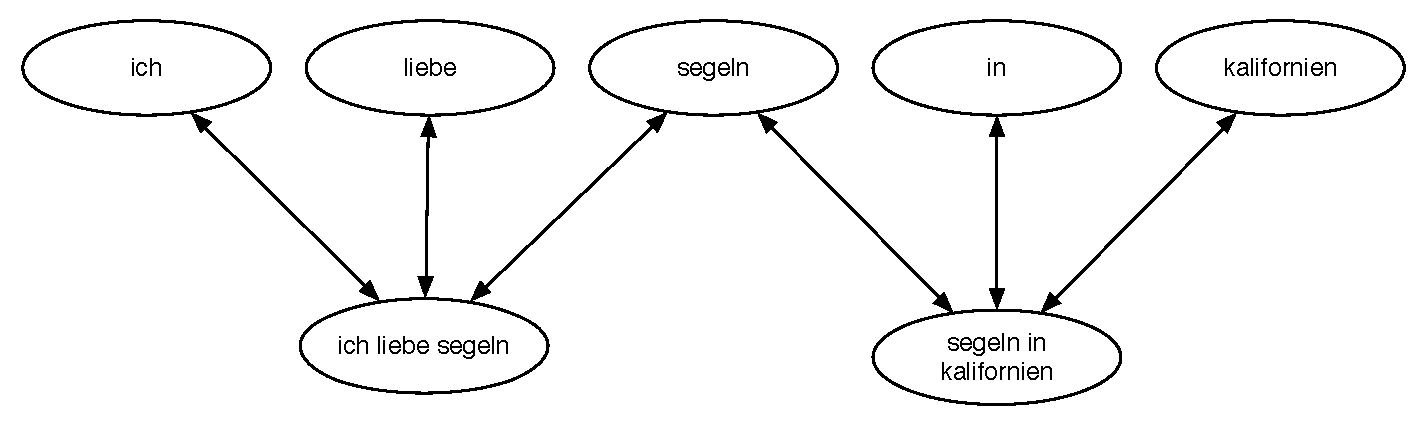
\includegraphics[width=\textwidth]{decomposition}
\caption{Beispielhafter Graphausschnitt nach der Zerlegung}
\label{fig:decomposition}
\end{figure}


\section{Wortschatz der Universität Leipzig}

Die Universität Leipzig betreibt ein Wortschatz-Projekt \cite{ws2013}. Im Rahmen dieses Projektes wird durch die Analyse von großen Textmengen eine Datenbank deutscher Wörter, deren Bedeutungen, grammatikalische Eigenschaften und Beziehungen zu anderen Wörtern aufgebaut.
\chapter{Optimierung und Evaluierung}

Im folgenden Kapitel werden die vorgenommenen Optimierungsmaßnahmen und die damit einhergehende Evaluierung der Ergebnisse der Link Discovery beschrieben. Dazu gehören der gewählte Ansatz zur Optimierung, eine Erläuterung evolutionärer Algorithmen und deren Einsatz zur Optimierung sowie die Darstellung und Auswertung der Ergebnisse.

\section{Optimierung}

Zuerst muss definiert werden, welcher Aspekt genau optimiert werden soll. Die in Kapitel \ref{link_discovery} beschriebenen Schritte haben einen Graphen erzeugt, in dem neun verschiedene Kantentypen existieren. Diese lauten \emph{Tag-Kookkurenz}, \emph{Klick-Kookkurenz}, \emph{Zusammensetzung}, \emph{Zerlegung}, \emph{Wortform}, \emph{Grundform}, \emph{Synonym}, \emph{Kategorie-Kookkurenz} und \emph{Thesaurus-Beziehung}.

Werden nun inhaltlich relevante Nachbarn zu einem gegebenen Begriff gesucht, müssen alle ausgehenden Kanten des entsprechenden Knotens nach Relevanz geordnet werden. Dazu muss jede Kante ein Kantengewicht besitzen. Die Addition aller Kantengewichte zwischen zwei Knoten stellt somit das Maß für ihre Nähe dar.

Die Kanten vom Typ Kookkurrenz besitzen bereits aufgrund der angegebenen Kookkurrenzmaße Kantengewichte. Jedoch muss hierbei festgelegt werden, welches Maß für das Kantengewicht herangezogen werden und in welchem Verhältnis zu den Gewichten anderer Kantentypen es stehen soll.

Somit hängt die Berechnung der Relevanz zwischen zwei Knoten von zwölf Parametern ab. Jedem Kantentyp muss ein Gewicht zugewiesen und außerdem muss eine Auswahl von drei Kookkurrenzmaßen getroffen werden. Die Optimierung und Evaluierung dieser berechneten Relevanz ist Gegenstand dieses Kapitels.

Die Einschätzung, ob die Ordnung der Nachbarn eine Ordnung der Relevanz zum Ausgangsbegriff darstellt, kann dabei nicht automatisch, sondern nur von Menschen, getroffen werden. Somit stellt die Bewertung einer bestimmten Gewichtung der Kanten auch eine Evaluierung der Kantentypen dar.
Generell kann außerdem nicht davon ausgegangen werden, dass eine einmal gefundene Gewichtung der Kanten für alle Knoten des Graphen verwertbare Ergebnisse erzeugt. Daher sollte die Optimierung nicht global, sondern für jeden Knoten einzeln erfolgen. Aufgrund der hohen Knotenanzahl wurde sich hierzu auf eine stichprobenartige Auswahl der Knotenmenge beschränkt.

Durch die Notwendigkeit menschlicher Beteiligung und der großen Anzahl an Parametern ist eine Optimierung mittels des Ausprobierens aller Fälle nicht möglich. Außerdem kann die Einschätzung, welche Kantengewichtungen relevante Ergebnisse erzeugen, stark von Mensch zu Mensch variieren. Stattdessen muss zur Optimierung ein Ansatz gefunden werden, der sich einer, für den Großteil der Personen, optimalen Gewichtung möglichst nähert. 

Im Rahmen dieser Arbeit wurde aus den genannten Gründen ein Optimierungsansatz mittels interaktiver evolutionärer Algorithmen gewählt. Die Grundlagen evolutionärer Algorithmen und die gewählte Implementierung werden in den folgenden Abschnitten beschrieben.

\section{Evolutionäre Algorithmen}

Als evolutionäre Algorithmen wird eine Klasse von Optimierungsverfahren bezeichnet, deren Funktionsweise an die Evolution natürlicher Lebewesen angelehnt ist. Sie versuchen, Probleme durch die Simulation von Evolution mittels der Auswahl der erfolgreichten Individuen zu lösen. Dabei kommen ebenfalls aus der Biologie entlehnte Mechanismen wie Mutation und Rekombination zum Einsatz, um iterativ eine Population von Lösungskandidaten zu verbessern \cite{tw2008}.

Es handelt sich dabei um heuristische Algorithmen, die das Finden einer optimalen Lösung nicht garantieren können.

Grundsätzlich folgt das Vorgehen dabei einem Kreislauf mit den Komponenten \emph{Evaluierung}, \emph{Selektion} und \emph{Reproduktion}. Nach Generierung einer anfänglichen Population (\emph{Initalisierung}) wird dieser Kreislauf so lange durchlaufen, bis ein vorher definiertes Abbruchkriterium eintritt. Ein Durchlauf wird dabei als \emph{Generation} bezeichnet. Das Abbruchkriterium kann beispielweise ein bestimmter Schwellwert für die Güte der Lösung oder eine feste Anzahl von Generationen sein. Der beschriebene Ablauf ist in Abbildung \ref{fig:evo_basic} dargestellt.

\begin{figure}
\centering
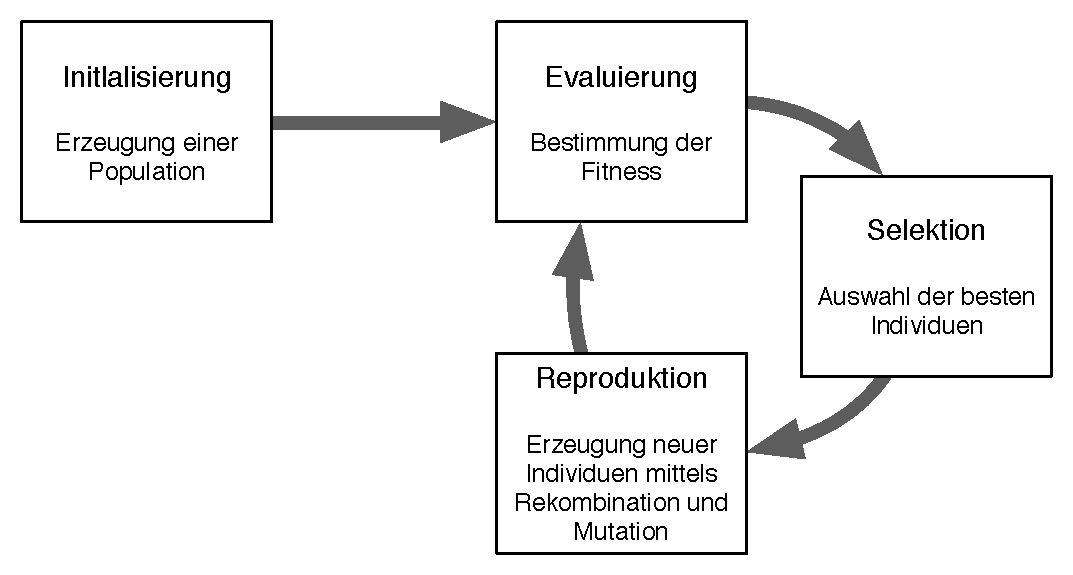
\includegraphics[width=0.8\textwidth]{evo_basic}
\caption{Ablauf evolutionärer Algorithmen}
\label{fig:evo_basic}
\end{figure}

Die einzelnen Komponenten eines evolutionären Algorithmus werden im Folgenden beschrieben. Die Definitionen folgen dabei im Wesentlichen denen von \textcite{tw2008}.

\paragraph{Initialisierung}

Die Population \(P\) stellt eine Menge von Lösungskandidaten dar. Ein Lösungskandidat \(i\) wird dabei als \emph{Individuum} bezeichnet und durch seinen \emph{Genotyp} repräsentiert. Der Genotyp ist die kodierte Repräsentation aller Variablen, die den Lösungskandidaten spezifizieren. Die Variablen werden \emph{Gene} genannt. Im Initlaisierungsschritt werden Lösungskandidaten erzeugt, die die Startpopulation des evolutionären Algorithmus bilden. Die Gene jedes Individuums werden dabei üblicherweise zufällig gewählt.

\paragraph{Evaluierung}

Der Evaluierungsschritt dient zur Bestimmung der \emph{Fitness} der Individuen, die noch in der Population enthalten sind. Die Fitness stellt dabei einen Wert dar, der die Güte der durch das Individuum repräsentierten Lösung bezüglich der Problemstellung beschreibt. Die Fitness kann dabei, je nach Optimierungsproblem, entweder absolut oder bezüglich der anderen Individuen der Population bestimmt werden. Somit lässt sich die Funktion zur Bestimmung der Fitness auf die Form \(fitness(i, P)\) generalisieren.

\paragraph{Selektion}

Im Selektionsschritt werden die fittesten Individuen der Population ausgewählt. Alle nicht ausgewählten Lösungskandidaten werden verworfen. Die Selektion kann dabei als Funktion der Form \(select(P, f, s)\) dargestellt werden, wobei \(s\) eine festgelegte Anzahl von Individuen darstellt, die ausgewählt werden sollen.

\paragraph{Reproduktion}

Die Reproduktion dient dazu, aus den im Selektionschritt ausgewählten Individuen neue Lösungskandidaten zu erzeugen. Dabei werden üblicherweise die Operationen \emph{Rekombination} und \emph{Mutation} verwendet. Eine Rekombination erzeugt dabei, analog zur Biologie, aus zwei Elternindividuen ein neues Kindindividuum. Sie lässt sich dabei als Funktion der Form \(i_n = recombine(i_a, i_b)\) darstellen, wobei \(i_n\) das neue Individuum und \(i_a\) und \(i_b\) die Elternindividuen darstellen. Eine Mutation erzeugt ein neues Individuen durch die Modifikation eines anderen und ist daher durch die Funktion \(i_n = mutate(i_a)\) spezifiziert.

In der Literatur \cite{kw2007, tw2008, dj2006} finden sich für Selektion, Mutation und Rekombination Standardverfahren, die in Hinblick auf das zu lösende Optimierungsproblem ausgewählt werden können. Wie die beschriebenen Schritte des evolutionären Algorithmus für die Optimierung der Link Discovery implementiert wurden, wird im folgenden Abschnitt beschrieben.

\section{Umsetzung}

Nachdem im vorhergehenden Abschnitt die Grundlagen und Komponenten evolutionärer Algorithmen beschrieben wurden, werden im Folgenden die für die Optimierung der Link Discovery-Ergebnnise angewendeten Methoden erläutert.

Zunächst soll die Methode zur Auswahl der Stichproben erläutert werden. Insgesamt wurden fünfzehn Knoten ausgewählt, deren Beziehungen optimiert werden sollen. Die Auswahl der Knoten richtete sich dabei nach der Popularität von Suchbegriffen auf der Spreadshirt-Plattform. Dazu wurden alle Begriffe mit mehr als eintausend Suchen herangezogen und diese nach Häufigkeit der Suchen geordnet. Daraus wurden zufällig je fünf Begriffe bis zum unteren Quartil, fünf Begriffe zwischen unterem und oberen Quartil und fünf Begriffe über dem oberen Quartil ausgewählt. Die ausgewählten Begriffe, deren Kantengewichtungen lokal optimiert werden sollen, lauten: \emph{Kopfkissenbezug}, \emph{Student}, \emph{Volkswagen}, \emph{Marathon}, \emph{Wow}, \emph{Krankenschwester}, \emph{Mountainbike}, \emph{Hammer}, \emph{Polska}, \emph{Regenbogen}, \emph{Minecraft}, \emph{Kind}, \emph{Dubstep}, \emph{Leipzig} und \emph{Valentinstag}.

Ziel dieser Auswahl war, eine möglichst vielfältige Verteilung der einzelnen Kantentypen zu erreichen, aus welcher sich nach Durchführung der Optimierung möglicherweise Erkenntnisse ableiten lassen, ob die Optimierung nur lokal oder auch global druchgeführt werden kann.

\section{Auswertung der Ergebnisse}
\chapter{Schlussbetrachtung}
\label{summary}

\section{Fazit}

\section{Ausblick}

\listoffigures
\listoftables
\lstlistoflistings

\sloppy
\printbibliography 

\appendix
\chapter{Ergebnisse der Priorisierung}
\label{other_results}

\begin{table}
\centering
\begin{tabular*}{0.9\textwidth}{@{\extracolsep{\fill} } lr}
    \toprule
    Begriff & Gewicht \\
    \midrule
    sex drugs dubstep & \num{0.58} \\
    dubstep beat & \num{0.58} \\
    dubstep music & \num{0.56} \\
    dubstep musik & \num{0.56} \\
    dubstep london & \num{0.56} \\
    \bottomrule
\end{tabular*}
\caption{Nachbarn des Begriffes ``Dubstep'' nach der Priorisierung}
\label{tab:prio_res_dubstep}
\end{table}

\begin{table}
\centering
\begin{tabular*}{0.9\textwidth}{@{\extracolsep{\fill} } lr}
    \toprule
    Begriff & Gewicht \\
    \midrule
    hämmern & \num{1.53} \\
    schlägel & \num{1.42} \\
    fäustel & \num{1.38} \\
    hammers & \num{1.34} \\
    klopfer & \num{1.33} \\
    \bottomrule
\end{tabular*}
\caption{Nachbarn des Begriffes ``Hammer'' nach der Priorisierung}
\label{tab:prio_res_hammer}
\end{table}

\begin{table}
\centering
\begin{tabular*}{0.9\textwidth}{@{\extracolsep{\fill} } lr}
    \toprule
    Begriff & Gewicht \\
    \midrule
    beautifulflower kopfkissenbezug & \num{0.93} \\
    ellipses kopfkissenbezug & \num{0.93} \\
    aurorae kopfkissenbezug & \num{0.93} \\
    chessboard kopfkissenbezug & \num{0.93} \\
    butterfly kopfkissenbezug & \num{0.93} \\
    \bottomrule
\end{tabular*}
\caption{Nachbarn des Begriffes ``Kopfkissenbezug'' nach der Priorisierung}
\label{tab:prio_res_kopfkissenbezug}
\end{table}

\begin{table}
\centering
\begin{tabular*}{0.9\textwidth}{@{\extracolsep{\fill} } lr}
    \toprule
    Begriff & Gewicht \\
    \midrule
    nurse & \num{1.06} \\
    arzt & \num{1.02} \\
    krankenpflegerin & \num{0.99} \\
    schwester & \num{0.92} \\
    krankenhaus & \num{0.91} \\
    \bottomrule
\end{tabular*}
\caption{Nachbarn des Begriffes ``Krankenschwester'' nach der Priorisierung}
\label{tab:prio_res_krankenschwester}
\end{table}

\begin{table}
\centering
\begin{tabular*}{0.9\textwidth}{@{\extracolsep{\fill} } lr}
    \toprule
    Begriff & Gewicht \\
    \midrule
    gutenberg marathon & \num{1.05} \\
    marathons & \num{1} \\
    laufe marathon & \num{0.98} \\
    berlin marathon & \num{0.98} \\
    vienna city marathon & \num{0.98} \\
    \bottomrule
\end{tabular*}
\caption{Nachbarn des Begriffes ``Marathon'' nach der Priorisierung}
\label{tab:prio_res_marathon}
\end{table}

\begin{table}
\centering
\begin{tabular*}{0.9\textwidth}{@{\extracolsep{\fill} } lr}
    \toprule
    Begriff & Gewicht \\
    \midrule
    creeper minecraft & \num{1.06} \\
    thegermanylp homies super minecraft pixel & \num{1} \\
    creeper girl minecraft sexy & \num{1} \\
    minecraft minetime mine craft & \num{1} \\
    geek gamer lol minecraft portal diablo spiel game fun tasse g4me & \num{1} \\
    \bottomrule
\end{tabular*}
\caption{Nachbarn des Begriffes ``Minecraft'' nach der Priorisierung}
\label{tab:prio_res_minecraft}
\end{table}

\begin{table}
\centering
\begin{tabular*}{0.9\textwidth}{@{\extracolsep{\fill} } lr}
    \toprule
    Begriff & Gewicht \\
    \midrule
    poland & \num{1.24} \\
    polen & \num{0.27} \\
    polish & \num{0.17} \\
    revolução & \num{0.15} \\
    rivoluzione & \num{0.15} \\
    \bottomrule
\end{tabular*}
\caption{Nachbarn des Begriffes ``Polska'' nach der Priorisierung}
\label{tab:prio_res_polska}
\end{table}

\begin{table}
\centering
\begin{tabular*}{0.9\textwidth}{@{\extracolsep{\fill} } lr}
    \toprule
    Begriff & Gewicht \\
    \midrule
    blitz & \num{3.07} \\
    regen & \num{2.49} \\
    blau & \num{2.48} \\
    wolke & \num{2.48} \\
    rot & \num{2.47} \\
    \bottomrule
\end{tabular*}
\caption{Nachbarn des Begriffes ``Regenbogen'' nach der Priorisierung}
\label{tab:prio_res_regenbogen}
\end{table}

\begin{table}
\centering
\begin{tabular*}{0.9\textwidth}{@{\extracolsep{\fill} } lr}
    \toprule
    Begriff & Gewicht \\
    \midrule
    schüler & \num{3.16} \\
    universität & \num{2.35} \\
    hochschule & \num{2.26} \\
    burschenschaft & \num{2.18} \\
    college & \num{2.17} \\
    \bottomrule
\end{tabular*}
\caption{Nachbarn des Begriffes ``Student'' nach der Priorisierung}
\label{tab:prio_res_student}
\end{table}

\begin{table}
\centering
\begin{tabular*}{0.9\textwidth}{@{\extracolsep{\fill} } lr}
    \toprule
    Begriff & Gewicht \\
    \midrule
    valentinstag t shirt & \num{1.06} \\
    alles gute zum valentinstag & \num{1.03} \\
    valentinstag geschenk & \num{1.02} \\
    ich hasse valentinstag & \num{1.01} \\
    ich liebe valentinstag & \num{1.01} \\
    \bottomrule
\end{tabular*}
\caption{Nachbarn des Begriffes ``Valentinstag'' nach der Priorisierung}
\label{tab:prio_res_valentinstag}
\end{table}

\begin{table}
\centering
\begin{tabular*}{0.9\textwidth}{@{\extracolsep{\fill} } lr}
    \toprule
    Begriff & Gewicht \\
    \midrule
    volkswagen bus & \num{1.1} \\
    volkswagen type 14 & \num{1.06} \\
    opel & \num{1.05} \\
    bus volkswagen & \num{1.04} \\
    volkswagen g60 & \num{1.04} \\
    \bottomrule
\end{tabular*}
\caption{Nachbarn des Begriffes ``Volkswagen'' nach der Priorisierung}
\label{tab:prio_res_volkswagen}
\end{table}

\begin{table}
\centering
\begin{tabular*}{0.9\textwidth}{@{\extracolsep{\fill} } lr}
    \toprule
    Begriff & Gewicht \\
    \midrule
    limitededition cool edition limitierte edition limited limitiert & \num{0.68} \\
    wow world of warcraft draenei & \num{0.68} \\
    wow gilde world of warcraft respawn kelthuzad & \num{0.68} \\
    chicken wow heiss chickeria & \num{0.68} \\
    wow mom & \num{0.68} \\
    \bottomrule
\end{tabular*}
\caption{Nachbarn des Begriffes ``Wow'' nach der Priorisierung}
\label{tab:prio_res_wow}
\end{table}

\end{document}